\chapter{Making Videos}

\section{Things to Keep in Mind}

\begin{itemize}
\item The  howtos in this  chapter assume that  you have a  correctly numbered
sequence of still frames, that you want  to turn into a movie. Such a sequence
is usually the result of creating an animation in one of the postprocessors.

\item We  primarily show  how to make  videos using ImageMagick,  mencoder and
ffmpeg  under Unix-like operating  systems. The  mentioned tools  already come
with  most Linux  distributions and  can be  installed from  the corresponding
package repositories.  We give hints for  installing the tools  on other OSes,
too.  It  is however only necessary  to either install mencoder  or ffmpeg for
most video formats, since both tools support mostly the same features.

\item Try to make sure that  the dimensions of your input frames are divisible
by 16, since 8x8  or 16x16 is the size of the  tiles many codecs usually apply
their FFTs or other transformations to.

\item Often PNG images cause a  problem as input frames for video encoders due
to  their alpha  channel  for transparency.  Use  the \texttt{-quality  100\%}
option to ImageMagick and convert the PNGs  to JPEGs, which do not have such a
channel.

\item The executbles of \texttt{ffmpeg} and \texttt{ffmpeg2theora} coming with
the  Miro Video  Converter can  be found  at  \texttt{/Applications/Miro Video
Converter.app/Contents/Resources} on the Mac.

\item  Some applications  (e.g. Internet  Explorer  9 or  Safari) and  devices
(e.g.  iPods)  natively  only  support  certain video  formats  with  hardware
acceleration (in the mentioned cases H.264 encoded video in .mp4 container).
\end{itemize}

% \subsection{Video Formats}
% .gif, .mng, .svg, etc

% % convert -delay 15 -loop 0 -transparent white -dispose previous fubar*.png fubar.mng

% \url{http://www.w3.org/TR/SVG/animate.html}
% \url{http://srufaculty.sru.edu/david.dailey/svg/}
% \url{https://developer.mozilla.org/en/SVG/SVG_animation_with_SMIL}
% \url{http://littlesvr.ca/apng/svg2png/examples/}
% \url{http://www.treebuilder.de/apng/aniSvgLogo2.svg}

% \url{http://wiki.inkscape.org/wiki/index.php/Animation-%28Timeline%29}
% \url{http://superuser.com/questions/358690/convert-animated-svg-to-animated-gif}
% \url{http://superuser.com/questions/48532/convert-animated-svg-to-movie}

\section{Tools}

\subsection{ImageMagick}

ImageMagick is  a software suite to  create, edit, compose,  or convert bitmap
images. It can read  and write images in a variety of  formats (over 100). The
functionality of  ImageMagick is typically  utilized from the command  line or
you   can  use   the  features   from  programs   written  in   your  favorite
language.  ImageMagick is  free software  delivered as  a  ready-to-run binary
distribution or  as source  code that  you may freely  use, copy,  modify, and
distribute in both open and proprietary applications.

\begin{description}
\item[ImageMagick Homepage] \url{http://www.imagemagick.org}
\item[Binary Releases (Win, Lin, Mac)] \url{http://www.imagemagick.org/script/binary-releases.php}
\item[Examples of ImageMagick Usage] \url{http://www.imagemagick.org/Usage/}
\item[Command-line Options] \url{http://www.imagemagick.org/script/command-line-options.php}
\item[Articles on IBM Developer Works]\footnote{Graphics from the Command Line: \url{http://www.ibm.com/developerworks/library/l-graf/?ca=dnt-428}\\
More graphics from the command line: \url{http://www.ibm.com/developerworks/library/l-graf2/?ca=dgr-lnxw15GraphicsLine}
}
\end{description}


\subsection{mplayer/mencoder}

MPlayer\footnote{MPlayer  website: \url{http://www.mplayerhq.hu}}  is  a movie
player which  runs on many  systems. Another great  feature of MPlayer  is the
wide range of supported output drivers.

\begin{description}
\item[MPlayer Download Page (Win, Lin, Mac)] \url{http://www.mplayerhq.hu/design7/dload.html}
\item[mplayer on MacPorts] \url{http://www.macports.org/ports.php?by=name&substr=mplayer}
\end{description}

\subsection{FFmpeg}

FFmpeg\footnote{FFmpeg  website:   \url{http://ffmpeg.org/}}  is  a  complete,
cross-platform solution  to record,  convert and stream  audio and  video.  It
includes libavcodec - the leading audio/video codec library.

\begin{description}
\item[Miro   Video   Converter]   ffmpeg   is   part   of   the   Miro   Video
Converter\footnote{Miro                    Video                    Converter:
\url{http://www.mirovideoconverter.com/}}  for  Mac  OS  X  and  Windows.  The
installation is quick  and simple and the program comes with  a simple GUI for
drag-and-drop video conversion.
\item[Binaries for Mac]\url{http://ffmpegmac.net/}
\item[ffmpeg on MacPorts] \url{http://www.macports.org/ports.php?by=name&substr=ffmpeg}
\end{description}

\section{Slideshow Programs}

\subsection{Microsoft PowerPoint 2003-2010}

\begin{description}
\item[Microsoft MPEGv2]  Files encoded with the msmpeg4v2  codec play natively
on every Windows since 2000. Maybe one has to rename the .avi file to .mpg.

% \item[WMV] WMV files should play on most Media Players.

\item[OGG Theora  Codec] If the  movies do not  work in Power Point  using the
DirectShow         component\footnote{Xiph        DirectShow        component:
\url{http://www.xiph.org/dshow}},    Theora\footnote{Theora    on   Wikipedia:
\url{http://de.wikipedia.org/wiki/Theora}} movies can  be played natively with
every  Firefox  browser  since  version 3.1\footnote{Theora  in  Firefox  3.1:
\url{http://www.linux-magazin.de/NEWS/Nativer-Ogg-Theora-Support-in-Firefox-3.1}}.

\item[Animated GIF]  Animated GIFs play natively  in Power Point  and in every
web browser on Windows.

\item[H.264 in .mp4 Container] Movie files encoded with the H.264 codec in the
.mp4  container format  are  natively  supported by  more  recent versions  of
Windows. They should also play in Internet Explorer 9.
\end{description}


\subsection{Microsoft PowerPoint 2011 for Mac}

\begin{description}
\item[H.264 in .mp4 Container] Movie files encoded with the H.264 codec in the
.mp4 container format are natively supported by Quicktime on MacOS X. They are
also natively supported on the latest Windows platforms.

\item[OGG  Theora Codec]  If the  movies do  not work  in Power  Point, Theora
movies  can  be played  natively  with  every  Firefox browser  since  version
3.1. Xiph QuickTime Components (XiphQT\footnote{Xiph components for QuickTime:
\url{http://xiph.org/quicktime}})  is,  in short,  the  solution  for Mac  and
Windows users who want to use Xiph formats in any QuickTime-based application,
e.g.  playing Ogg Vorbis in iTunes or producing Ogg Theora with iMovie.

\item[Animated GIF]  Animated GIFs play natively  in Power Point  and in every
web browser on Mac.

\item[Microsoft  MPEGv2]  Files encoded  with  the  msmpeg4v2  codec need  the
Perian\footnote{Perian website: \url{http://perian.org}} codec pack to play on
Mac.

%\item[WMV       on       Mac]       Flip4Mac\footnote{Flip4Mac       website:
%\url{http://www.telestream.net/flip4mac-wmv/overview.htm}} WMV  is required to
% play these files.
\end{description}

\section{Video Howtos}

\subsection{Extraction of Still Frames From a Video}

The following  commands extract eight seconds  of video frames  starting at 22
seconds from  the input video into a  sequence of PNG image  files.  This also
works for extracting single frames from animated GIFs.

\begin{verbatim}
mplayer input.mp4 -ss 0:00:22 -endpos 0:00:30 -nosound -vo png:z=0

ffmpeg -i input.mp4 -ss 00:00:22 -t 8 -y img-%04d.png
\end{verbatim}%
%
In order to extract the frames from an animated GIF one may type

\begin{verbatim}
convert anim.gif frame_%d.png 
\end{verbatim}%
%
For a certain frame the command is
\begin{verbatim}
convert anim.gif[0] frame_0.png 
\end{verbatim}

\subsection{Replacing Background Color in Still Frames}

The following  ImageMagick command  replaces all pixels  having the same  or a
15\% similar color like pixel 5x5 with white color.
 
\begin{verbatim}
convert -fill white -draw 'color 5,5 replace' \
        -fuzz 15% anim.0001.png out.png
\end{verbatim}%
%
Make background transparent
\begin{verbatim}
convert anim.0020.png -matte -fill none -draw 'matte 0,0 floodfill' out.png
\end{verbatim}

\subsection{Batch Processing}

There are many ways  to process all files in a directory  in one shot. You can
use the unix  shell utils \texttt{find} and \texttt{xargs}.   Suppose you want
to convert all files in a dir from png to jpg.  Here's GNU/Linux example:

\begin{verbatim}
find . -name "anim.00*.png" | xargs -l -i basename ".png" "{}" | \
    xargs -l -i convert -quality 85% "{}.png" "{}.jpg"
\end{verbatim}%
%
The \texttt{-l} makes it process one line at a time. The \texttt{-i} makes the
\texttt{\{\}}  to  stand  for  file  name. The  \texttt{basename}  strips  the
suffix.%
%
Another alternative is to use a for loop
\begin{verbatim}
for f in anim.00*.png; do \
    convert -quality 85% $f $(echo $f|sed 's/\.png/\.jpg/g'); \
done
\end{verbatim}%
%
The  \texttt{mogrify} tool  from  ImageMagick works  on  a list  of files  and
accepts the same arguments as \texttt{convert}
\begin{verbatim}
mogrify -format jpg -quality 85% anim.00*.png
\end{verbatim}%
%
Often files are numbered in a wrong  way and have to be renumbered for further
automatic processing. This may be achieved using

\inputminted{shell}{sources/batch_renumber_files.txt}

\subsection{Obtaining Infos From Movies and Stills}

ImageMagick    contains   the    tool   \texttt{identify}\footnote{ImageMagick
\texttt{identify}  tool: \url{http://www.imagemagick.org/script/identify.php}}
which can  be used to query information  from images and movies.  An even more
advanced  tool for  performing such  operations  is ExifTool\footnote{ExifTool
website: \url{http://owl.phy.queensu.ca/~phil/exiftool/}}

\subsection{Cropping and Repaging Frames}

The following  examples show how to crop  away borders from and  to resize the
frames  in  an  animation.   The  most  general solution  for  this  is  again
ImageMagick\footnote{Resizing       to      Fill      a       Given      Space
\url{http://www.imagemagick.org/Usage/resize/\#space_fill}}   but  almost  the
same results  can be  achieved using FFmpeg\footnote{ffmpeg  libavfilter Video
Filters:             \url{http://ffmpeg.org/libavfilter.html}}             and
mencoder\footnote{Mencoder                    Video                   Filters:
\url{http://www.mplayerhq.hu/DOCS/man/en/mplayer.1.html\#VIDEO\%20FILTERS}}
(cf. Fig. \ref{fig:video_crop}).

\begin{verbatim}
convert anim.0020.png -crop 810x428+10+156 +repage \
        -fill violet -draw 'color 5,5 floodfill' -resize 400x300\> \
        -size 400x300 xc:blue +swap -gravity center -composite out.png
\end{verbatim}

\begin{verbatim}
VFOPTS="crop=810:428:10:156"
VFOPTS="$VFOPTS,scale=400:-1"
VFOPTS="$VFOPTS,pad=400:300:(ow-iw)/2:(oh-ih)/2:violet"

ffmpeg -i anim.0020.png -vf "$VFOPTS" out2.png
\end{verbatim}

\begin{verbatim}
mencoder "mf://anim*.png" -mf fps=10 -ffourcc MP42 -o test.avi \
         -ovc lavc -lavcopts vcodec=msmpeg4v2:vbitrate=3000:vhq 
         -vf 'crop=810:428:10:156,scale=400:-2,expand=0:300'
\end{verbatim}

\begin{figure}[htb] 
  \centering 
  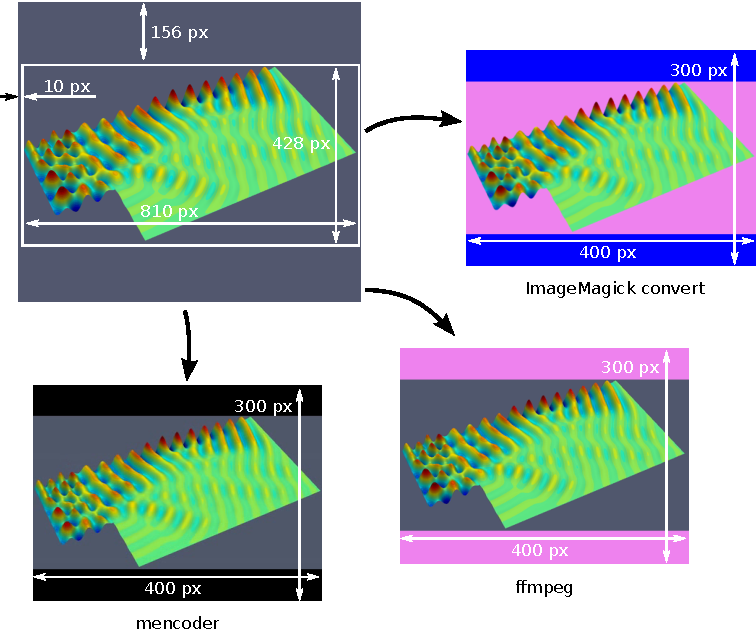
\includegraphics[height=8cm]{pics/video_crop}
  \caption{Cropping and repaging video frames.}
  \label{fig:video_crop}
\end{figure}

\subsection{Creating the Video}

\begin{description}
\item[Animated GIF]

Creating animated  GIFs works best with  ImageMagick.  It is  also possible to
create them using ffmpeg or  mencoder but the results using default parameters
look much worse.
\begin{verbatim}
convert -verbose -delay 20 -loop 0 -matte -fill none \
        -draw 'matte 0,0 floodfill' \
        -dispose previous anim.00* output.gif
\end{verbatim}

\item[Microsoft MPEG4v2  Codec for Win2K until  Win7] It is  important to also
set     the    correct    FOURCC     code\footnote{FOURCC.org    website:
\url{http://www.fourcc.org}} for the videos to play correctly
\begin{verbatim}
ffmpeg -f image2 -r 15 -i ./anim.%04d.png -vcodec msmpeg4v2 \
       -qscale 1 -vtag MP42 filename.avi

mencoder "mf://anim*.png" -mf fps=10 -ffourcc MP42 -o test.avi \
         -ovc lavc -lavcopts vcodec=msmpeg4v2:vbitrate=3000:vhq
\end{verbatim}

\item[Ogg    Theora]    The   ffmpeg2theora    encoder\footnote{ffmpeg2theora:
\url{http://v2v.cc/~j/ffmpeg2theora/}}  obviously has  problems  with PNGs  as
input, therefore we convert them to JPEGs with the same quality.
\begin{verbatim}
mogrify -format jpg -quality 100% anim.00*.png
ffmpeg2theora -f image2 anim.%4d.jpg --optimize --videoquality 10 \
              --inputfps 15 -o output.ogv
\end{verbatim}

\item[H.264 in  .mp4 Container] We make sure  that we have JPEGs  as input and
then apply a set  of high quality options to FFmpeg, which  have been found by
googling, .

\begin{verbatim}
for f in anim.00*.png; do
  convert $f -crop 810x428+10+156 +repage -quality 100% \
          $(echo $f|sed 's/\.png/\.jpg/g');
done

ffmpeg -y -i anim.%04d.jpg -vcodec libx264 \
       -vf 'scale=640:-1,pad=640:480:(ow-iw)/2:(oh-ih)/2:black' \
       -level 41 -crf 20 -bufsize 20000k -maxrate 25000k -g 250 \
       -r 20 -coder 1 -flags +loop -cmp +chroma \
       -partitions +parti4x4+partp8x8+partb8x8 -flags2 +dct8x8+bpyramid \
       -me_method umh -subq 7 -me_range 16 -keyint_min 25 -sc_threshold 40 \
       -i_qfactor 0.71 -rc_eq 'blurCplx^(1-qComp)' -bf 16 -b_strategy 1 \
       -bidir_refine 1 -refs 6 -deblockalpha 0 -deblockbeta 0 output.mp4
\end{verbatim}

\end{description}

\section{Further Reading}

Scientific Movie Howto\footnote{Scientific Movie Howto: \url{http://solarmuri.ssl.berkeley.edu/~fisher/public/manuscripts/scientific-movie-HOWTO.txt}}

\subsection{Embedding Videos in HTML5}

Safari won’t  support Ogg Theora and  Firefox and Opera won’t  support H.264 —
doesn’t  mean you  can’t support  all three  browsers. It  just means  that to
support    all    three,    you    need    to    include    at    least    two
\texttt{{\textless}source{\textgreater}}       elements       within       the
\texttt{{\textless}video{\textgreater}} tag, one  pointing to an H.264-encoded
file,   the  other   to   an  Ogg   Theora   file,  like   this\footnote{HTML5
\texttt{{\textless}video{\textgreater}}                                    tag:
\url{http://www.w3schools.com/html5/html5_video.asp}\\    Using    the   HTML5
\texttt{{\textless}video{\textgreater}}    tag   with   a    Flash   fallback:
\url{http://henriksjokvist.net/archive/2009/2/using-the-html5-video-tag-with-a-flash-fallback}\\
HTML5                    Audio                    and                   Video:
\url{http://www.html5tuts.co.uk/tutorials/audioandvideo/} }:

\begin{verbatim}
<!DOCTYPE html>
<html>
<body>

<video width="480" height="320" controls="controls">
  <!-- MPEG4 for Safari -->
  <source src="example-video.mp4" type="video/mp4" /> 
  <!-- Ogg Theora for Firefox 3.1b2 --> 
  <source src="example-video.ogv" type="video/ogg" /> 

  <img alt="animated GIF" src="example-video.gif" width="480" height="320" />
  Your browser does not support the video tag. Falling back to animated GIF.
</video>

</body>
</html>
\end{verbatim}%
%
Currently,  the the  \texttt{{\textless}video{\textgreater}}  element supports
the video formats MP4, WebM, and Ogg:
\begin{description}
\item[MP4] MPEG 4 files with H264 video codec and AAC audio codec
\item[WebM] WebM files with VP8 video codec and Vorbis audio codec
\item[Ogg] Ogg files with Theora video codec and Vorbis audio codec
\end{description}

\begin{table}[htb]
\centering
\begin{minipage}[h]{0.9\textwidth}\caption{Video Formats and Browser Support.}
\label{tab:web_browser_video_formats}
\end{minipage}
\par\medskip\noindent
\begin{minipage}[h]{0.9\textwidth}
\centering
\begin{tabular}{lccc}
  \toprule
  {\bf Browser}             & {\bf MP4} & {\bf WebM} & {\bf Ogg} \\ \otoprule
  {\bf Internet Explorer 9} &	YES     &    NO      & NO   \\
  {\bf Firefox 4.0}         &   NO      &    YES     & YES  \\
  {\bf Google Chrome 6}     &   YES     &    YES     & YES  \\
  {\bf Apple Safari 5}      &   YES     &    NO      & NO   \\
  {\bf Opera 10.6}          &   NO      &    YES     & YES  \\
  \bottomrule
\end{tabular} 
\end{minipage}
\end{table}
